\part{XML}


\chapter{Overview}


XML(Extensible Markup Language,可扩展标记语言)是一种标记语言。

标记本身是指计算机所能理解的信息符号,通过此种标记,计算机之间可以处理包含各种信息的文章等。

如何定义这些标记,既可以选择国际通用的标记语言(比如HTML),也可以使用像XML这样由相关人士自由决定的标记语言,这就是语言的可扩展性。

XML是从标准通用标记语言(SGML)中简化修改出来的,主要用到的有可扩展标记语言(XML)、可扩展样式语言(XSL)、XBRL和XPath等。

XML是从1995年开始有其雏形,并向W3C(万维网联盟)提案,并在1998年二月发布为W3C的标准(XML1.0)。

XML的前身GML(The Standard Generalized Markup Language)是自IBM从1960年代就开始发展的GML(Generalized Markup Language)标准化后的名称,SGML的问题在于其本身是一种非常严谨的文件描述法,导致过于庞大复杂,难以理解和学习,进而影响其推广与应用。

GML提出了两个重要概念,分别是:

\begin{compactitem}
\item 文件中能够明确的将标示与内容分开
\item 所有文件的标示使用方法均一致
\end{compactitem}

1978年,ANSI将GML加以整理规范,发布成为SGML,1986年起为ISO所采用(ISO 8879),并且被广泛地运用在各种大型的文件计划中。

对于SGML的竞争对手HTML,W3C也提到了HTML的问题:

\begin{compactitem}
\item 不能解决所有解释数据的问题(例如影音文件或化学公式、音乐符号等其他形态的内容)。
\item 性能问题 - 需要下载整份文件,才能开始对文件做搜索。
\item 扩充性、弹性、易读性均不佳。
\end{compactitem}

为了解决以上问题,专家们使用SGML精简制作,并依照HTML的发展经验,产生出一套使用上规则严谨但是简单的描述数据语言——XML。


XML是在一个这样的背景下诞生的——为了有一个更中立的方式,让消费端自行决定要如何消化、呈现从服务端所提供的信息,后来XML被广泛用来作为跨平台之间交互数据的形式(主要针对数据的内容),通过不同的格式化描述手段(XSLT,CSS等)可以完成最终的形式表达(生成对应的HTML,PDF或者其他的文件格式)。

和HTML相比,XML被设计用来传送及携带数据信息,不用来表现或展示数据,HTML语言则用来表现数据,所以XML用途的焦点是它说明数据是什么,以及携带数据信息。

下面是RecipeBook(一种基于XML语法上的烹饪技术书刊)的例子,此标签可转换为HTML、PDF以及Rich Text Format并使用编程语言或XSL。
\begin{figure}[htbp]
\centering
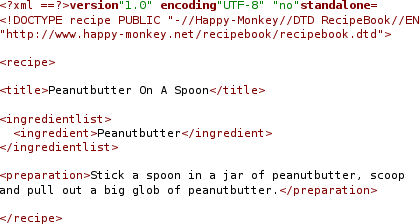
\includegraphics[scale=0.3]{RecipeBook_XML_Example}
\caption{RecipeBook示例}
\end{figure}



\begin{compactitem}
\item 富文本(Rich Documents)- 自定文件描述并使其更丰富,例如属于文件为主的XML技术应用中,标记用来定义一份资料应该如何呈现。

\item 元数据(Metadata)- 描述其它文件或网络信息,例如属于资料为主的XML技术应用中,标记是用来说明一份资料的意义。

\item 配置文档(Configuration Files)- 描述软件设置的参数

\end{compactitem}

下面的示例为小张发送给大元的便条(存储为XML),可以看出XML定义结构、存储信息、传送信息,XML文档仅是纯粹的信息标签,这些标签意义的展开依赖于应用它的程序。

\begin{lstlisting}[language=XML]
<?xml version =“1.0”?>
<小纸条>
  <收件人>大元</
  <发件人>小张</发件人>
  <主题>问候</主题>
  <具体内容>早啊,饭吃了没?</具体内容>
</小纸条>
\end{lstlisting}


每个XML文档都由XML序言开始,在前面的代码中的第一行就是XML序言,\texttt{<?xml version="1.0"?>},这一行代码会告诉解析器或浏览器这个文件应该按照XML规则进行解析。


不过,根元素到底叫<小纸条>还是<Book>则是由文档类型定义(DTD)或XML纲要定义的。如果DTD规定根元素必须叫<小便条>,那么写作<小纸条>就不匹配要求。这种不匹配DTD或XML纲要的要求的XML文档,被称作不合法的XML,反之则是合法的XML。


XML文件的第二行并不一定要包含文档元素;如果有注释或者其他内容,文档元素可以迟些出现。


这个PI一般会直接放在XML序言之后,通常由Web浏览器使用,来将XML数据以特殊的样式显示出来。

注意,XML的结构有一个缺陷,那就是不支持分帧(framing)。例如,当多条XML消息在TCP上传输的时候,无法基于XML协议来确定一条XML消息是否已经结束。


\section{DOM}


\section{libxml}


\section{SDO}


\section{SDO-DAS-Relational}


\section{SDO-DAS-XML}


\section{SimpleXML}


\section{WDDX}


\section{XMLDiff}


\section{XML Parser}


\section{XMLReader}


\section{XMLWriter}


\section{XSL}


\chapter{DOM}

\section{Overview}


DOM扩展允许开发者通过DOM API来操作XML文档,PHP默认启用DOM扩展(可以通过\texttt{-\/-disable-dom}禁用)。

DOM默认使用UTF-8编码,开发者可以使用utf8\_encode()和utf8\_decode()来处理ISO-8859-1编码的文本或者使用iconv扩展来处理其他编码格式。

下面的DOM示例使用的book.xml示例文件如下:

\begin{lstlisting}[language=XML]
<?xml version="1.0" encoding="utf-8"?>
<!DOCTYPE book PUBLIC "-//OASIS//DTD DocBook XML V4.1.2//EN"
 "http://www.oasis-open.org/docbook/xml/4.1.2/docbookx.dtd" [
]>
<book id="listing">
 <title>My lists</title>
 <chapter id="books">
  <title>My books</title>
  <para>
   <informaltable>
    <tgroup cols="4">
     <thead>
      <row>
       <entry>Title</entry>
       <entry>Author</entry>
       <entry>Language</entry>
       <entry>ISBN</entry>
      </row>
     </thead>
     <tbody>
      <row>
       <entry>The Grapes of Wrath</entry>
       <entry>John Steinbeck</entry>
       <entry>en</entry>
       <entry>0140186409</entry>
      </row>
      <row>
       <entry>The Pearl</entry>
       <entry>John Steinbeck</entry>
       <entry>en</entry>
       <entry>014017737X</entry>
      </row>
      <row>
       <entry>Samarcande</entry>
       <entry>Amine Maalouf</entry>
       <entry>fr</entry>
       <entry>2253051209</entry>
      </row>
      <!-- TODO: I have a lot of remaining books to add.. -->
     </tbody>
    </tgroup>
   </informaltable>
  </para>
 </chapter>
</book>
\end{lstlisting}


\subsection{Requirement}

DOM和SimpleXML都需要libxml扩展的支持,因此在编译PHP时需要指定\texttt{-\/-enable-libxml},不过实际上libxml默认是开启的。

\begin{lstlisting}[language=bash]
$ php --ri libxml
libxml

libXML support => active
libXML Compiled Version => 2.9.1
libXML Loaded Version => 20901
libXML streams => enabled
\end{lstlisting}


\subsection{Resource Type}

DOM没有定义资源类型。


\subsection{Build-in Module}

DOM默认为启用,可以在编译时通过如下选项禁用\texttt{-\/-disable-dom}。

如果需要手动安装XML扩展,可以执行:

\begin{lstlisting}[language=bash]
$ sudo apt-get install php7.0-xml
\end{lstlisting}



\subsection{Runtime Configure}

DOM没有在 php.ini 中定义配置指令。





\subsection{Predefined Constants}

DOM提供了自己的预定义常量,并且仅在DOM扩展编译入PHP或者在运行时动态载入DOM扩展时可用。


\zihao{6}
\begin{longtable}{|m{150pt}|m{40pt}|m{120pt}|}
%head
\multicolumn{3}{r}{}
\tabularnewline\hline
常量名&常量值&说明
\endhead
%endhead

%firsthead
\caption{DOM扩展的预定义常量}\\
\hline
常量名&常量值&说明
\endfirsthead
%endfirsthead

%foot
\multicolumn{3}{r}{}
\endfoot
%endfoot

%lastfoot
\endlastfoot
%endlastfoot
\hline
XML\_ELEMENT\_NODE (integer)		&1		&Node is a DOMElement\\
\hline
XML\_ATTRIBUTE\_NODE (integer)	&2		&Node is a DOMAttr\\
\hline
XML\_TEXT\_NODE (integer)		&3		&Node is a DOMText\\
\hline
XML\_CDATA\_SECTION\_NODE (integer)&4	&Node is a DOMCharacterData\\
\hline
XML\_ENTITY\_REF\_NODE (integer)	&5		&Node is a DOMEntityReference\\
\hline
XML\_ENTITY\_NODE (integer)		&6		&Node is a DOMEntity\\
\hline
XML\_PI\_NODE (integer)			&7		&Node is a DOMProcessingInstruction\\
\hline
XML\_COMMENT\_NODE (integer)	&8		&Node is a DOMComment\\
\hline
XML\_DOCUMENT\_NODE (integer)	&9		&Node is a DOMDocument\\
\hline
XML\_DOCUMENT\_TYPE\_NODE (integer)&10	&Node is a DOMDocumentType\\
\hline
XML\_DOCUMENT\_FRAG\_NODE (integer)&11	&Node is a DOMDocumentFragment\\
\hline
XML\_NOTATION\_NODE (integer)	&12		&Node is a DOMNotation\\
\hline
XML\_HTML\_DOCUMENT\_NODE (integer)&13 &	 \\
\hline
XML\_DTD\_NODE (integer)			&14	 	&\\
\hline
XML\_ELEMENT\_DECL\_NODE (integer)&15	& \\
\hline
XML\_ATTRIBUTE\_DECL\_NODE (integer)&16	& \\
\hline
XML\_ENTITY\_DECL\_NODE (integer)	&17	 	&\\
\hline
XML\_NAMESPACE\_DECL\_NODE (integer)	&18	& \\
\hline
XML\_ATTRIBUTE\_CDATA (integer)	&1	 	&\\
\hline
XML\_ATTRIBUTE\_ID (integer)		&2	 	&\\
\hline
XML\_ATTRIBUTE\_IDREF (integer)	&3	 	&\\
\hline
XML\_ATTRIBUTE\_IDREFS (integer)	&4	 	&\\
\hline
XML\_ATTRIBUTE\_ENTITY (integer)	&5	 	&\\
\hline
XML\_ATTRIBUTE\_NMTOKEN (integer)&7	 	&\\
\hline
XML\_ATTRIBUTE\_NMTOKENS (integer)&8	& \\
\hline
XML\_ATTRIBUTE\_ENUMERATION (integer)&9	& \\
\hline
XML\_ATTRIBUTE\_NOTATION (integer)	&10	&\\
\hline
\end{longtable}


\begin{longtable}{|m{150pt}|m{40pt}|m{200pt}|}
%head
\multicolumn{3}{r}{}
\tabularnewline\hline
常量名&常量值&说明
\endhead
%endhead

%firsthead
\caption{DOMException的预定义常量}\\
\hline
常量名&常量值&说明
\endfirsthead
%endfirsthead

%foot
\multicolumn{3}{r}{}
\endfoot
%endfoot

%lastfoot
\endlastfoot
%endlastfoot
\hline
DOM\_PHP\_ERR (integer)					&0	&Error code not part of the DOM specification. Meant for PHP errors.\\
\hline
DOM\_INDEX\_SIZE\_ERR (integer)			&1	&If index or size is negative, or greater than the allowed value.\\
\hline
DOMSTRING\_SIZE\_ERR (integer)			&2	&If the specified range of text does not fit into a DOMString.\\
\hline
DOM\_HIERARCHY\_REQUEST\_ERR (integer)	&3	&If any node is inserted somewhere it doesn't belong\\
\hline
DOM\_WRONG\_DOCUMENT\_ERR (integer)	&4	&If a node is used in a different document than the one that created it.\\
\hline
DOM\_INVALID\_CHARACTER\_ERR (integer)	&5	&If an invalid or illegal character is specified, such as in a name.\\
\hline
DOM\_NO\_DATA\_ALLOWED\_ERR (integer)	&6	&If data is specified for a node which does not support data.\\
\hline
DOM\_NO\_MODIFICATION\_ALLOWED\_ERR (integer)&7&If an attempt is made to modify an object where modifications are not allowed.\\
\hline
DOM\_NOT\_FOUND\_ERR (integer)			&8	&If an attempt is made to reference a node in a context where it does not exist.\\
\hline
DOM\_NOT\_SUPPORTED\_ERR (integer)		&9	&If the implementation does not support the requested type of object or operation.\\
\hline
DOM\_INUSE\_ATTRIBUTE\_ERR (integer)		&10	&If an attempt is made to add an attribute that is already in use elsewhere.\\
\hline
DOM\_INVALID\_STATE\_ERR (integer)		&11	&If an attempt is made to use an object that is not, or is no longer, usable.\\
\hline
DOM\_SYNTAX\_ERR (integer)				&12	&If an invalid or illegal string is specified.\\
\hline
DOM\_INVALID\_MODIFICATION\_ERR (integer)	&13	&If an attempt is made to modify the type of the underlying object.\\
\hline
DOM\_NAMESPACE\_ERR (integer)			&14	&If an attempt is made to create or change an object in a way which is incorrect with regard to namespaces.\\
\hline
DOM\_INVALID\_ACCESS\_ERR (integer)		&15	&If a parameter or an operation is not supported by the underlying object.\\
\hline
DOM\_VALIDATION\_ERR (integer)			&16	&If a call to a method such as insertBefore or removeChild would make the Node invalid with respect to "partial validity", this exception would be raised and the operation would not be done.\\
\hline
\end{longtable}


\zihao{5}

\section{DOMAttr}


DOMAttr表示DOMElement对象中的一个属性。


\begin{lstlisting}[language=PHP]
DOMAttr extends DOMNode {
    /* 属性 */
    public readonly string $name ;
    public readonly DOMElement $ownerElement ;
    public readonly bool $schemaTypeInfo ;
    public readonly bool $specified ;
    public string $value ;
    /* 方法 */
    public __construct ( string $name [, string $value ] )
    public bool isId ( void )
    /* 继承的方法 */
    public DOMNode DOMNode::appendChild ( DOMNode $newnode )
    public string DOMNode::C14N ([ bool $exclusive [, bool $with_comments [, array $xpath [, array $ns_prefixes ]]]] )
    public int DOMNode::C14NFile ( string $uri [, bool $exclusive [, bool $with_comments [, array $xpath [, array $ns_prefixes ]]]] )
    public DOMNode DOMNode::cloneNode ([ bool $deep ] )
    public int DOMNode::getLineNo ( void )
    public string DOMNode::getNodePath ( void )
    public bool DOMNode::hasAttributes ( void )
    public bool DOMNode::hasChildNodes ( void )
    public DOMNode DOMNode::insertBefore ( DOMNode $newnode [, DOMNode $refnode ] )
    public bool DOMNode::isDefaultNamespace ( string $namespaceURI )
    public bool DOMNode::isSameNode ( DOMNode $node )
    public bool DOMNode::isSupported ( string $feature , string $version )
    public string DOMNode::lookupNamespaceURI ( string $prefix )
    public string DOMNode::lookupPrefix ( string $namespaceURI )
    public void DOMNode::normalize ( void )
    public DOMNode DOMNode::removeChild ( DOMNode $oldnode )
    public DOMNode DOMNode::replaceChild ( DOMNode $newnode , DOMNode $oldnode )
}
\end{lstlisting}

\subsection{\$name}

\$name是XML属性的名称

\subsection{\$ownerElement}

\$ownerElement是包含XML属性的XML元素

\subsection{\$schemaTypeInfo}

\$schemaTypeInfo未实现,总是返回NULL。

\subsection{\$specified}

\$specified未实现,总是返回NULL。

\subsection{\$value}

\$value是XML属性的值。

\subsection{DOMAttr::\_\_construct()}

创建一个新的只读的DOMAttr对象。

\begin{lstlisting}[language=PHP]
public DOMAttr::__construct ( string $name [, string $value ] )
\end{lstlisting}

创建新的DOMAttr对象,而且这个DOMAttr对象是只读的,可以被附加到XML文档,但是额外的节点直到该节点与XML文档相关联时才可以不附加到该节点。 


要创建可写节点,可以使用DOMDocument::createAttribute()。

\begin{compactitem}
\item \$name - 属性的tag名字
\item \$value - 属性的值
\end{compactitem}



\begin{lstlisting}[language=PHP]
<?php
$dom = new DOMDocument('1.0','iso-8859-1');
$element = $dom->appendChild(new DOMElement('root'));
$attr = $element->setAttributeNode(new DOMAttr('attr','attrvalue'));
echo $dom->saveXML();

// 以上例程会输出:
<?xml version="1.0" encoding="iso-8859-1"?>
<root attr="attrvalue" />
\end{lstlisting}


\begin{lstlisting}[language=PHP]

\end{lstlisting}



\subsection{DOMAttr::isId()}

检查一个XML属性是否是一个已定义的ID。

\begin{lstlisting}[language=PHP]
public bool DOMAttr::isId ( void )
\end{lstlisting}

isId()函数检查属性是否是定义的ID,成功时返回 TRUE, 或者在失败时返回 FALSE。

根据DOM标准,这需要将属性ID定义为ID类型的DTD。 在使用此函数之前,您需要使用DOMDocument::validate或DOMDocument::validateOnParse来验证XML文档。



\begin{lstlisting}[language=PHP]
<?php
$doc = new DomDocument;
// validate xml document before refering to the id
$doc->validateOnParse = true;
$doc->Load('book.xml');

// retrieve the attribute named id of the chapter element
$attr = $doc->getElementsByTagName('chapter')->item(0)->getAttributeNode('id');
var_dump($attr->isId()); // bool(true)
\end{lstlisting}


\section{DOMCdataSection}



DOMCdataSection继承自DOMText,用于CData结构的文本化表示。

\begin{lstlisting}[language=PHP]
DOMCdataSection extends DOMText {
    /* Methods */
    public __construct ( string $value )
    /* Inherited methods */
    public bool DOMText::isWhitespaceInElementContent ( void )
    public DOMText DOMText::splitText ( int $offset )
}
\end{lstlisting}


\subsection{DOMCdataSection::\_\_construct()}


构造新的DOMCdataSection对象


\begin{lstlisting}[language=PHP]
public DOMCdataSection::__construct ( string $value )
\end{lstlisting}

构造一个新的CDATA节点,其过程类似于DOMText类。

\begin{compactitem}
\item \$value - CDATA节点的值。如果没有提供,那么会创建一个新的空的CDATA节点。
\end{compactitem}


\begin{lstlisting}[language=PHP]
<?php
$dom = new DOMDocument('1.0', 'utf-8');
$element = $dom->appendChild(new DOMElement('root'));
$text = $element->appendChild(new DOMCdataSection('root value'));
echo $dom->saveXML();
// 以上例程会输出:
// <?xml version="1.0" encoding="utf-8"?>
// <root><![CDATA[root value]]></root>
\end{lstlisting}




\section{DOMCharacterData}

表示具有字符数据的节点。 没有节点直接对应这个类,但其他节点从它继承。



\begin{lstlisting}[language=PHP]
DOMCharacterData extends DOMNode {
    /* 属性 */
    public string $data ;
    readonly public int $length ;
    /* 方法 */
    void appendData ( string $data )
    void deleteData ( int $offset , int $count )
    void insertData ( int $offset , string $data )
    void replaceData ( int $offset , int $count , string $data )
    string substringData ( int $offset , int $count )
    /* 继承的方法 */
    public DOMNode DOMNode::appendChild ( DOMNode $newnode )
    public string DOMNode::C14N ([ bool $exclusive [, bool $with_comments [, array $xpath [, array $ns_prefixes ]]]] )
    public int DOMNode::C14NFile ( string $uri [, bool $exclusive [, bool $with_comments [, array $xpath [, array $ns_prefixes ]]]] )
    public DOMNode DOMNode::cloneNode ([ bool $deep ] )
    public int DOMNode::getLineNo ( void )
    public string DOMNode::getNodePath ( void )
    public bool DOMNode::hasAttributes ( void )
    public bool DOMNode::hasChildNodes ( void )
    public DOMNode DOMNode::insertBefore ( DOMNode $newnode [, DOMNode $refnode ] )
    public bool DOMNode::isDefaultNamespace ( string $namespaceURI )
    public bool DOMNode::isSameNode ( DOMNode $node )
    public bool DOMNode::isSupported ( string $feature , string $version )
    public string DOMNode::lookupNamespaceURI ( string $prefix )
    public string DOMNode::lookupPrefix ( string $namespaceURI )
    public void DOMNode::normalize ( void )
    public DOMNode DOMNode::removeChild ( DOMNode $oldnode )
    public DOMNode DOMNode::replaceChild ( DOMNode $newnode , DOMNode $oldnode )
}
\end{lstlisting}

\subsection{\$data}

XML节点的内容


\subsection{\$length}

XML节点内容的长度

\subsection{DOMCharacterData::appendData()}

将字符串附加到节点的字符数据的结尾


\begin{lstlisting}[language=PHP]
void DOMCharacterData::appendData ( string $data )
\end{lstlisting}

在XML节点的字符末尾追加\$data变量中的字符串值。

\begin{compactitem}
\item \$data - 要追加的字符串
\end{compactitem}



\subsection{DOMCharacterData::deleteData()}

从节点中删除一定范围的字符

\begin{lstlisting}[language=PHP]
void DOMCharacterData::deleteData ( int $offset , int $count )
\end{lstlisting}

从XML节点的\$offset指定的偏移开始删除\$count个字符。

\begin{compactitem}
\item \$offset - 开始删除字符的偏移。


\item \$count - 要删除的字符个数。
\end{compactitem}

如果\$offset和\$count超过长度,那么节点中到末尾的数据都会删除。

如果\$offset或\$count是负数,或者大于数据中的16位单元的总长度,deleteData()都会抛出DOM\_INDEX\_SIZE\_ERR错误。


\subsection{DOMCharacterData::insertData()}

以指定的16位单位偏移插入一个字符串

\begin{lstlisting}[language=PHP]
void DOMCharacterData::insertData ( int $offset , string $data )
\end{lstlisting}

从\$offset指定的位置开始插入字符串数据\$data。

\begin{compactitem}
\item \$offset - 开始插入字符串的偏移位置
\item \$data - 要插入的字符串
\end{compactitem}

如果\$offset或者大于数据中的16位单元的总长度,insertData()都会抛出DOM\_INDEX\_SIZE\_ERR错误。

\subsection{DOMCharacterData::replaceData()}

替换DOMCharacterData节点中的子字符串

\begin{lstlisting}[language=PHP]
void DOMCharacterData::replaceData ( int $offset , int $count , string $data )
\end{lstlisting}

从\$offset指定的位置开始,使用\$data的数据替换\$count个字符。

\begin{compactitem}
\item \$offset - 开始替换字符的偏移位置
\item \$count - 要替换字符的个数
\item \$data - 要替换已有的的字符串数据
\end{compactitem}

如果\$offset和\$count超过长度,那么节点中到末尾的数据都会被替换。

如果\$offset或\$count是负数或者大于数据中的16位单元的总长度,replaceData()都会抛出DOM\_INDEX\_SIZE\_ERR错误。



\subsection{DOMCharacterData::substringData()}

从节点提取一系列数据

\begin{lstlisting}[language=PHP]
string DOMCharacterData::substringData ( int $offset , int $count )
\end{lstlisting}

返回指定的子字符串。

\begin{compactitem}
\item \$offset - 需要提取子字符串的开始偏移位置
\item \$count - 需要提取子字符串的字符个数
\end{compactitem}


如果\$offset和\$count超过长度,那么将会返回直到末尾的所有数据的16位单元。

如果\$offset或\$count是负数或者大于数据中的16位单元的总长度,substringData()都会抛出DOM\_INDEX\_SIZE\_ERR错误。



\section{DOMComment}

输出注释节点,由\texttt{<!-\/-} 和\texttt{-\/->}分隔的字符。



\begin{lstlisting}[language=PHP]
DOMComment extends DOMCharacterData {
    /* 方法 */
    public __construct ([ string $value ] )
    /* 继承的方法 */
    void DOMCharacterData::appendData ( string $data )
    void DOMCharacterData::deleteData ( int $offset , int $count )
    void DOMCharacterData::insertData ( int $offset , string $data )
    void DOMCharacterData::replaceData ( int $offset , int $count , string $data )
    string DOMCharacterData::substringData ( int $offset , int $count )
    public DOMNode DOMNode::appendChild ( DOMNode $newnode )
    public string DOMNode::C14N ([ bool $exclusive [, bool $with_comments [, array $xpath [, array $ns_prefixes ]]]] )
    public int DOMNode::C14NFile ( string $uri [, bool $exclusive [, bool $with_comments [, array $xpath [, array $ns_prefixes ]]]] )
    public DOMNode DOMNode::cloneNode ([ bool $deep ] )
    public int DOMNode::getLineNo ( void )
    public string DOMNode::getNodePath ( void )
    public bool DOMNode::hasAttributes ( void )
    public bool DOMNode::hasChildNodes ( void )
    public DOMNode DOMNode::insertBefore ( DOMNode $newnode [, DOMNode $refnode ] )
    public bool DOMNode::isDefaultNamespace ( string $namespaceURI )
    public bool DOMNode::isSameNode ( DOMNode $node )
    public bool DOMNode::isSupported ( string $feature , string $version )
    public string DOMNode::lookupNamespaceURI ( string $prefix )
    public string DOMNode::lookupPrefix ( string $namespaceURI )
    public void DOMNode::normalize ( void )
    public DOMNode DOMNode::removeChild ( DOMNode $oldnode )
    public DOMNode DOMNode::replaceChild ( DOMNode $newnode , DOMNode $oldnode )
}
\end{lstlisting}

\subsection{DOMComment::\_\_construct()}

创建一个新的DOMComment对象。

\begin{lstlisting}[language=PHP]
public DOMComment::__construct ([ string $value ] )
\end{lstlisting}

创建新的DOMComment对象,而且对象是只读的,可以被附加到XML文档,但是附加节点可以不附加到该节点,直到该节点与文档相关联。

要创建可写节点,需要使用DOMDocument::createComment()。

\begin{compactitem}
\item \$value - XML Comment的值
\end{compactitem}


\begin{lstlisting}[language=PHP]
<?php
$dom = new DOMDocument('1.0','iso-8859-1');
$element = $dom->appendChild(new DOMElement('root'));
$comment = $element->appendChild(new DOMComment('root comment'));
echo $dom->saveXML(); 
// 返回结果如下:
// <?xml version="1.0" encoding="iso-8859-1"?>
//   <root><!--root comment--></root>
\end{lstlisting}



\section{DOMDocument}

表示整个HTML或XML文档; 用作文档树的根。


\begin{lstlisting}[language=PHP]
DOMDocument extends DOMNode {
     /* 属性 */
     readonly public string $actualEncoding ;
     readonly public DOMConfiguration $config ;
     readonly public DOMDocumentType $doctype ;
     readonly public DOMElement $documentElement ;
     public string $documentURI ;
     public string $encoding ;
     public bool $formatOutput ;
     readonly public DOMImplementation $implementation ;
     public bool $preserveWhiteSpace = true ;
     public bool $recover ;
     public bool $resolveExternals ;
     public bool $standalone ;
     public bool $strictErrorChecking = true ;
     public bool $substituteEntities ;
     public bool $validateOnParse = false ;
     public string $version ;
     readonly public string $xmlEncoding ;
     public bool $xmlStandalone ;
     public string $xmlVersion ;
     /* 方法 */
     public __construct ([ string $version [, string $encoding ]] )
     public DOMAttr createAttribute ( string $name )
     public DOMAttr createAttributeNS ( string $namespaceURI , string $qualifiedName )
     public DOMCDATASection createCDATASection ( string $data )
     public DOMComment createComment ( string $data )
     public DOMDocumentFragment createDocumentFragment ( void )
     public DOMElement createElement ( string $name [, string $value ] )
     public DOMElement createElementNS ( string $namespaceURI , string $qualifiedName [, string $value ] )
     public DOMEntityReference createEntityReference ( string $name )
     public DOMProcessingInstruction createProcessingInstruction ( string $target [, string $data ] )
     public DOMText createTextNode ( string $content )
     public DOMElement getElementById ( string $elementId )
     public DOMNodeList getElementsByTagName ( string $name )
     public DOMNodeList getElementsByTagNameNS ( string $namespaceURI , string $localName )
     public DOMNode importNode ( DOMNode $importedNode [, bool $deep ] )
     public mixed load ( string $filename [, int $options = 0 ] )
     public bool loadHTML ( string $source [, int $options = 0 ] )
     public bool loadHTMLFile ( string $filename [, int $options = 0 ] )
     public mixed loadXML ( string $source [, int $options = 0 ] )
     public void normalizeDocument ( void )
     public bool registerNodeClass ( string $baseclass , string $extendedclass )
     public bool relaxNGValidate ( string $filename )
     public bool relaxNGValidateSource ( string $source )
     public int save ( string $filename [, int $options ] )
     public string saveHTML ([ DOMNode $node = NULL ] )
     public int saveHTMLFile ( string $filename )
     public string saveXML ([ DOMNode $node [, int $options ]] )
     public bool schemaValidate ( string $filename [, int $flags ] )
     public bool schemaValidateSource ( string $source [, int $flags ] )
     public bool validate ( void )
     public int xinclude ([ int $options ] )
     /* 继承的方法 */
     public DOMNode DOMNode::appendChild ( DOMNode $newnode )
     public string DOMNode::C14N ([ bool $exclusive [, bool $with_comments [, array $xpath [, array $ns_prefixes ]]]] )
     public int DOMNode::C14NFile ( string $uri [, bool $exclusive [, bool $with_comments [, array $xpath [, array $ns_prefixes ]]]] )
     public DOMNode DOMNode::cloneNode ([ bool $deep ] )
     public int DOMNode::getLineNo ( void )
     public string DOMNode::getNodePath ( void )
     public bool DOMNode::hasAttributes ( void )
     public bool DOMNode::hasChildNodes ( void )
     public DOMNode DOMNode::insertBefore ( DOMNode $newnode [, DOMNode $refnode ] )
     public bool DOMNode::isDefaultNamespace ( string $namespaceURI )
     public bool DOMNode::isSameNode ( DOMNode $node )
     public bool DOMNode::isSupported ( string $feature , string $version )
     public string DOMNode::lookupNamespaceURI ( string $prefix )
     public string DOMNode::lookupPrefix ( string $namespaceURI )
     public void DOMNode::normalize ( void )
     public DOMNode DOMNode::removeChild ( DOMNode $oldnode )
     public DOMNode DOMNode::replaceChild ( DOMNode $newnode , DOMNode $oldnode )
}
\end{lstlisting}


\subsection{\$actualEncoding}

Deprecated. Actual encoding of the document, is a readonly equivalent to encoding.

\subsection{\$config}

Deprecated. Configuration used when DOMDocument::normalizeDocument() is invoked.

\subsection{\$doctype}

The Document Type Declaration associated with this document.

\subsection{\$documentElement}

This is a convenience attribute that allows direct access to the child node that is the document element of the document.

\subsection{\$documentURI}

The location of the document or NULL if undefined.

\subsection{\$encoding}

Encoding of the document, as specified by the XML declaration. This attribute is not present in the final DOM Level 3 specification, but is the only way of manipulating XML document encoding in this implementation.

\subsection{\$formatOutput}

Nicely formats output with indentation and extra space.

\subsection{\$implementation}

The DOMImplementation object that handles this document.

\subsection{\$preserveWhiteSpace}

Do not remove redundant white space. Default to TRUE.

\subsection{\$recover}

Proprietary. Enables recovery mode, i.e. trying to parse non-well formed documents. This attribute is not part of the DOM specification and is specific to libxml.

\subsection{\$resolveExternals}

Set it to TRUE to load external entities from a doctype declaration. This is useful for including character entities in your XML document.

\subsection{\$standalone}

Deprecated. Whether or not the document is standalone, as specified by the XML declaration, corresponds to xmlStandalone.

\subsection{\$strictErrorChecking}

Throws DOMException on errors. Default to TRUE.

\subsection{\$substituteEntities}

Proprietary. Whether or not to substitute entities. This attribute is not part of the DOM specification and is specific to libxml.

\subsection{\$validateOnParse}

Loads and validates against the DTD. Default to FALSE.

\subsection{\$version}

Deprecated. Version of XML, corresponds to xmlVersion.

\subsection{\$xmlEncoding}

An attribute specifying, as part of the XML declaration, the encoding of this document. This is NULL when unspecified or when it is not known, such as when the Document was created in memory.

\subsection{\$xmlStandalone}

An attribute specifying, as part of the XML declaration, whether this document is standalone. This is FALSE when unspecified.

\subsection{\$xmlVersion}

An attribute specifying, as part of the XML declaration, the version number of this document. If there is no declaration and if this document supports the "XML" feature, the value is "1.0".

\subsection{DOMDocument::\_\_construct()}


\begin{lstlisting}[language=PHP]

\end{lstlisting}


\subsection{DOMDocument::createAttribute()}



\begin{lstlisting}[language=PHP]

\end{lstlisting}

\subsection{DOMDocument::createAttributeNS()}



\begin{lstlisting}[language=PHP]

\end{lstlisting}

\subsection{DOMDocument::createCDATASection()}



\begin{lstlisting}[language=PHP]

\end{lstlisting}


\subsection{DOMDocument::createComment()}





\begin{lstlisting}[language=PHP]

\end{lstlisting}


\subsection{DOMDocument::createDocumentFragment()}



\begin{lstlisting}[language=PHP]

\end{lstlisting}

\subsection{DOMDocument::createElement()}



\begin{lstlisting}[language=PHP]

\end{lstlisting}

\subsection{DOMDocument::createElementNS()}



\begin{lstlisting}[language=PHP]

\end{lstlisting}

\subsection{DOMDocument::createEntityReference()}


\begin{lstlisting}[language=PHP]

\end{lstlisting}


\subsection{DOMDocument::createProcessingInstruction()}

\begin{lstlisting}[language=PHP]

\end{lstlisting}

\subsection{DOMDocument::createTextNode()}


\begin{lstlisting}[language=PHP]

\end{lstlisting}

\subsection{DOMDocument::getElementById()}

\begin{lstlisting}[language=PHP]

\end{lstlisting}

\subsection{DOMDocument::getElementsByTagName()}


\begin{lstlisting}[language=PHP]

\end{lstlisting}

\subsection{DOMDocument::getElementsByTagNameNS()}



\begin{lstlisting}[language=PHP]

\end{lstlisting}


\subsection{DOMDocument::importNode()}

\begin{lstlisting}[language=PHP]

\end{lstlisting}

\subsection{DOMDocument::load()}

\begin{lstlisting}[language=PHP]

\end{lstlisting}

\subsection{DOMDocument::loadHTML()}

\begin{lstlisting}[language=PHP]

\end{lstlisting}

\subsection{DOMDocument::loadHTMLFile()}


\begin{lstlisting}[language=PHP]

\end{lstlisting}


\subsection{DOMDocument::normalizeDocument()}



\begin{lstlisting}[language=PHP]

\end{lstlisting}


\subsection{DOMDocument::registerNodeClass()}

\begin{lstlisting}[language=PHP]

\end{lstlisting}


\subsection{DOMDocument::relaxNGValidate()}


\begin{lstlisting}[language=PHP]

\end{lstlisting}


\subsection{DOMDocument::relaxNGValidateSource()}


\begin{lstlisting}[language=PHP]

\end{lstlisting}


\subsection{DOMDocument::save()}


\begin{lstlisting}[language=PHP]

\end{lstlisting}


\subsection{DOMDocument::saveHTML()}


\begin{lstlisting}[language=PHP]

\end{lstlisting}

\subsection{DOMDocument::saveHTMLFile()}


\begin{lstlisting}[language=PHP]

\end{lstlisting}

\subsection{DOMDocument::saveXML()}


\begin{lstlisting}[language=PHP]

\end{lstlisting}


\subsection{DOMDocument::schemaValidate()}


\begin{lstlisting}[language=PHP]

\end{lstlisting}


\subsection{DOMDocument::schemaValidateSource()}


\begin{lstlisting}[language=PHP]

\end{lstlisting}


\subsection{DOMDocument::validate()}


\begin{lstlisting}[language=PHP]

\end{lstlisting}


\subsection{DOMDocument::xinclude()}












\section{DOMDocumentFragment}


\begin{lstlisting}[language=PHP]
DOMDocumentFragment extends DOMNode {
    /* 属性 */
    /* 方法 */
    public bool appendXML ( string $data )
    /* 继承的方法 */
    public DOMNode DOMNode::appendChild ( DOMNode $newnode )
    public string DOMNode::C14N ([ bool $exclusive [, bool $with_comments [, array $xpath [, array $ns_prefixes ]]]] )
    public int DOMNode::C14NFile ( string $uri [, bool $exclusive [, bool $with_comments [, array $xpath [, array $ns_prefixes ]]]] )
    public DOMNode DOMNode::cloneNode ([ bool $deep ] )
    public int DOMNode::getLineNo ( void )
    public string DOMNode::getNodePath ( void )
    public bool DOMNode::hasAttributes ( void )
    public bool DOMNode::hasChildNodes ( void )
    public DOMNode DOMNode::insertBefore ( DOMNode $newnode [, DOMNode $refnode ] )
    public bool DOMNode::isDefaultNamespace ( string $namespaceURI )
    public bool DOMNode::isSameNode ( DOMNode $node )
    public bool DOMNode::isSupported ( string $feature , string $version )
    public string DOMNode::lookupNamespaceURI ( string $prefix )
    public string DOMNode::lookupPrefix ( string $namespaceURI )
    public void DOMNode::normalize ( void )
    public DOMNode DOMNode::removeChild ( DOMNode $oldnode )
    public DOMNode DOMNode::replaceChild ( DOMNode $newnode , DOMNode $oldnode )
}
\end{lstlisting}

\subsection{DOMDocumentFragment::appendXML()}

追加原始XML数据。


\begin{lstlisting}[language=PHP]
public bool DOMDocumentFragment::appendXML ( string $data )
\end{lstlisting}


将原始XML数据附加到DOMDocumentFragment,成功时返回 TRUE, 或者在失败时返回 FALSE。

此方法不是DOM标准的一部分。 它被创建为一个更简单的方法在DOMDocument中附加一个XML DocumentFragment。

如果需要遵循标准,必须创建一个临时DOMDocument与一个虚拟根,然后循环通过XML数据根的子节点来附加它们。

\begin{compactitem}
\item \$data - 要追加的XML数据
\end{compactitem}



\begin{lstlisting}[language=PHP]
<?php
$doc = new DOMDocument();
$doc->loadXML('<root/>');
$f = $doc->createDocmentFragment();
$f->appendXML('<foo>text1</foo><bar>text2</bar>');
$doc->documentElement->appendChild($f);
echo $doc->saveXML();
// 以上例程会输出:
// <?xml version="1.0"?>
// <root><foo>text1</foo><bar>text2</bar></root>
\end{lstlisting}



\section{DOMDocumentType}

每个DOMDocument都有一个doctype属性,其值为NULL或DOMDocumentType对象。

\begin{lstlisting}[language=PHP]
DOMDocumentType extends DOMNode {
    /* 属性 */
    readonly public string $publicId ;
    readonly public string $systemId ;
    readonly public string $name ;
    readonly public DOMNamedNodeMap $entities ;
    readonly public DOMNamedNodeMap $notations ;
    readonly public string $internalSubset ;
    /* 继承的方法 */
    public DOMNode DOMNode::appendChild ( DOMNode $newnode )
    public string DOMNode::C14N ([ bool $exclusive [, bool $with_comments [, array $xpath [, array $ns_prefixes ]]]] )
    public int DOMNode::C14NFile ( string $uri [, bool $exclusive [, bool $with_comments [, array $xpath [, array $ns_prefixes ]]]] )
    public DOMNode DOMNode::cloneNode ([ bool $deep ] )
    public int DOMNode::getLineNo ( void )
    public string DOMNode::getNodePath ( void )
    public bool DOMNode::hasAttributes ( void )
    public bool DOMNode::hasChildNodes ( void )
    public DOMNode DOMNode::insertBefore ( DOMNode $newnode [, DOMNode $refnode ] )
    public bool DOMNode::isDefaultNamespace ( string $namespaceURI )
    public bool DOMNode::isSameNode ( DOMNode $node )
    public bool DOMNode::isSupported ( string $feature , string $version )
    public string DOMNode::lookupNamespaceURI ( string $prefix )
    public string DOMNode::lookupPrefix ( string $namespaceURI )
    public void DOMNode::normalize ( void )
    public DOMNode DOMNode::removeChild ( DOMNode $oldnode )
    public DOMNode DOMNode::replaceChild ( DOMNode $newnode , DOMNode $oldnode )
}
\end{lstlisting}

\subsection{\$publicId}

\begin{lstlisting}[language=PHP]

\end{lstlisting}


\subsection{\$systemId}



\begin{lstlisting}[language=PHP]

\end{lstlisting}

\subsection{\$name}



\begin{lstlisting}[language=PHP]

\end{lstlisting}

\subsection{\$entities}



\begin{lstlisting}[language=PHP]

\end{lstlisting}

\subsection{\$notations}


\begin{lstlisting}[language=PHP]

\end{lstlisting}

\subsection{\$internalSubset}

\section{DOMElement}


\begin{lstlisting}[language=PHP]
DOMElement extends DOMNode {
   /* 属性 */
   readonly public bool $schemaTypeInfo ;
   readonly public string $tagName ;
   /* 方法 */
   public __construct ( string $name [, string $value [, string $namespaceURI ]] )
   public string getAttribute ( string $name )
   public DOMAttr getAttributeNode ( string $name )
   public DOMAttr getAttributeNodeNS ( string $namespaceURI , string $localName )
   public string getAttributeNS ( string $namespaceURI , string $localName )
   public DOMNodeList getElementsByTagName ( string $name )
   public DOMNodeList getElementsByTagNameNS ( string $namespaceURI , string $localName )
   public bool hasAttribute ( string $name )
   public bool hasAttributeNS ( string $namespaceURI , string $localName )
   public bool removeAttribute ( string $name )
   public bool removeAttributeNode ( DOMAttr $oldnode )
   public bool removeAttributeNS ( string $namespaceURI , string $localName )
   public DOMAttr setAttribute ( string $name , string $value )
   public DOMAttr setAttributeNode ( DOMAttr $attr )
   public DOMAttr setAttributeNodeNS ( DOMAttr $attr )
   public void setAttributeNS ( string $namespaceURI , string $qualifiedName , string $value )
   public void setIdAttribute ( string $name , bool $isId )
   public void setIdAttributeNode ( DOMAttr $attr , bool $isId )
   public void setIdAttributeNS ( string $namespaceURI , string $localName , bool $isId )
   /* 继承的方法 */
   public DOMNode DOMNode::appendChild ( DOMNode $newnode )
   public string DOMNode::C14N ([ bool $exclusive [, bool $with_comments [, array $xpath [, array $ns_prefixes ]]]] )
   public int DOMNode::C14NFile ( string $uri [, bool $exclusive [, bool $with_comments [, array $xpath [, array $ns_prefixes ]]]] )
   public DOMNode DOMNode::cloneNode ([ bool $deep ] )
   public int DOMNode::getLineNo ( void )
   public string DOMNode::getNodePath ( void )
   public bool DOMNode::hasAttributes ( void )
   public bool DOMNode::hasChildNodes ( void )
   public DOMNode DOMNode::insertBefore ( DOMNode $newnode [, DOMNode $refnode ] )
   public bool DOMNode::isDefaultNamespace ( string $namespaceURI )
   public bool DOMNode::isSameNode ( DOMNode $node )
   public bool DOMNode::isSupported ( string $feature , string $version )
   public string DOMNode::lookupNamespaceURI ( string $prefix )
   public string DOMNode::lookupPrefix ( string $namespaceURI )
   public void DOMNode::normalize ( void )
   public DOMNode DOMNode::removeChild ( DOMNode $oldnode )
   public DOMNode DOMNode::replaceChild ( DOMNode $newnode , DOMNode $oldnode )
}
\end{lstlisting}

\subsection{\$schemaTypeInfo}

\begin{lstlisting}[language=PHP]

\end{lstlisting}

\subsection{\$tagName}


\begin{lstlisting}[language=PHP]

\end{lstlisting}

\subsection{DOMElement::\_\_construct()}


\begin{lstlisting}[language=PHP]

\end{lstlisting}

\subsection{DOMElement::getAttribute()}

\begin{lstlisting}[language=PHP]

\end{lstlisting}

\subsection{DOMElement::getAttributeNode()}

\begin{lstlisting}[language=PHP]

\end{lstlisting}

\subsection{DOMElement::getAttributeNodeNS()}

\begin{lstlisting}[language=PHP]

\end{lstlisting}

\subsection{DOMElement::getElementsByTagName()}

\begin{lstlisting}[language=PHP]

\end{lstlisting}

\subsection{DOMElement::getElementsByTagNameNS()}

\begin{lstlisting}[language=PHP]

\end{lstlisting}

\subsection{DOMElement::hasAttribute()}

\begin{lstlisting}[language=PHP]

\end{lstlisting}

\subsection{DOMElement::hasAttributeNS()}

\begin{lstlisting}[language=PHP]

\end{lstlisting}

\subsection{DOMElement::removeAttribute()}

\begin{lstlisting}[language=PHP]

\end{lstlisting}


\subsection{DOMElement::removeAttributeNode()}

\begin{lstlisting}[language=PHP]

\end{lstlisting}

\subsection{DOMElement::removeAttributeNS()}

\begin{lstlisting}[language=PHP]

\end{lstlisting}

\subsection{DOMElement::setAttribute()}

\begin{lstlisting}[language=PHP]

\end{lstlisting}

\subsection{DOMElement::setAttributeNode()}

\begin{lstlisting}[language=PHP]

\end{lstlisting}


\subsection{DOMDocument::setAttributeNodeNS()}

\begin{lstlisting}[language=PHP]

\end{lstlisting}

\subsection{DOMDocument::setAttributeNS()}

\begin{lstlisting}[language=PHP]

\end{lstlisting}


\subsection{DOMDocument::setIdAttribute()}


\begin{lstlisting}[language=PHP]

\end{lstlisting}


\subsection{DOMDocument::setIdAttributeNode()}


\begin{lstlisting}[language=PHP]

\end{lstlisting}


\subsection{DOMDocument::setIdAttributeNS()}

\begin{lstlisting}[language=PHP]

\end{lstlisting}









\section{DOMEntity}

DOMEntity接口表示XML文档中已解析或未解析的已知实体。


\begin{lstlisting}[language=PHP]
DOMEntity extends DOMNode {
/* 属性 */
readonly public string $publicId ;
readonly public string $systemId ;
readonly public string $notationName ;
public string $actualEncoding ;
readonly public string $encoding ;
readonly public string $version ;
/* 继承的方法 */
public DOMNode DOMNode::appendChild ( DOMNode $newnode )
public string DOMNode::C14N ([ bool $exclusive [, bool $with_comments [, array $xpath [, array $ns_prefixes ]]]] )
public int DOMNode::C14NFile ( string $uri [, bool $exclusive [, bool $with_comments [, array $xpath [, array $ns_prefixes ]]]] )
public DOMNode DOMNode::cloneNode ([ bool $deep ] )
public int DOMNode::getLineNo ( void )
public string DOMNode::getNodePath ( void )
public bool DOMNode::hasAttributes ( void )
public bool DOMNode::hasChildNodes ( void )
public DOMNode DOMNode::insertBefore ( DOMNode $newnode [, DOMNode $refnode ] )
public bool DOMNode::isDefaultNamespace ( string $namespaceURI )
public bool DOMNode::isSameNode ( DOMNode $node )
public bool DOMNode::isSupported ( string $feature , string $version )
public string DOMNode::lookupNamespaceURI ( string $prefix )
public string DOMNode::lookupPrefix ( string $namespaceURI )
public void DOMNode::normalize ( void )
public DOMNode DOMNode::removeChild ( DOMNode $oldnode )
public DOMNode DOMNode::replaceChild ( DOMNode $newnode , DOMNode $oldnode )
}
\end{lstlisting}


\subsection{\$pupblidId}


\begin{lstlisting}[language=PHP]

\end{lstlisting}

\subsection{\$systemId}

\begin{lstlisting}[language=PHP]

\end{lstlisting}

\subsection{\$notationName}

\begin{lstlisting}[language=PHP]

\end{lstlisting}

\subsection{\$actualEncoding}


\begin{lstlisting}[language=PHP]

\end{lstlisting}

\subsection{\$encoding}


\begin{lstlisting}[language=PHP]

\end{lstlisting}


\subsection{\$version}


\section{DOMEntityReference}


\begin{lstlisting}[language=PHP]
DOMEntityReference extends DOMNode {
/* 属性 */
/* 方法 */
public __construct ( string $name )
/* 继承的方法 */
public DOMNode DOMNode::appendChild ( DOMNode $newnode )
public string DOMNode::C14N ([ bool $exclusive [, bool $with_comments [, array $xpath [, array $ns_prefixes ]]]] )
public int DOMNode::C14NFile ( string $uri [, bool $exclusive [, bool $with_comments [, array $xpath [, array $ns_prefixes ]]]] )
public DOMNode DOMNode::cloneNode ([ bool $deep ] )
public int DOMNode::getLineNo ( void )
public string DOMNode::getNodePath ( void )
public bool DOMNode::hasAttributes ( void )
public bool DOMNode::hasChildNodes ( void )
public DOMNode DOMNode::insertBefore ( DOMNode $newnode [, DOMNode $refnode ] )
public bool DOMNode::isDefaultNamespace ( string $namespaceURI )
public bool DOMNode::isSameNode ( DOMNode $node )
public bool DOMNode::isSupported ( string $feature , string $version )
public string DOMNode::lookupNamespaceURI ( string $prefix )
public string DOMNode::lookupPrefix ( string $namespaceURI )
public void DOMNode::normalize ( void )
public DOMNode DOMNode::removeChild ( DOMNode $oldnode )
public DOMNode DOMNode::replaceChild ( DOMNode $newnode , DOMNode $oldnode )
}
\end{lstlisting}


\subsection{DOMEntityReference::\_\_construct()}

\begin{lstlisting}[language=PHP]

\end{lstlisting}


\begin{lstlisting}[language=PHP]

\end{lstlisting}


\begin{lstlisting}[language=PHP]

\end{lstlisting}


\begin{lstlisting}[language=PHP]

\end{lstlisting}


\begin{lstlisting}[language=PHP]

\end{lstlisting}
\section{DOMException}

DOM操作在特定情况下(即当由于逻辑原因而不可能执行操作时)引发DOMException异常。


\begin{lstlisting}[language=PHP]
DOMException extends Exception {
/* 属性 */
readonly public int $code ;
/* 继承的方法 */
final public string Exception::getMessage ( void )
final public Exception Exception::getPrevious ( void )
final public int Exception::getCode ( void )
final public string Exception::getFile ( void )
final public int Exception::getLine ( void )
final public array Exception::getTrace ( void )
final public string Exception::getTraceAsString ( void )
public string Exception::__toString ( void )
final private void Exception::__clone ( void )
}
\end{lstlisting}

\subsection{\$code}


\begin{lstlisting}[language=PHP]

\end{lstlisting}


\begin{lstlisting}[language=PHP]

\end{lstlisting}


\begin{lstlisting}[language=PHP]

\end{lstlisting}


\begin{lstlisting}[language=PHP]

\end{lstlisting}


\begin{lstlisting}[language=PHP]

\end{lstlisting}
\section{DOMImplementation}


DOMImplementation接口提供了许多用于执行独立于文档对象模型的任何特定实例的操作的方法。

\begin{lstlisting}[language=PHP]
DOMImplementation {
/* 属性 */
/* 方法 */
__construct ( void )
public DOMDocument createDocument ([ string $namespaceURI = NULL [, string $qualifiedName = NULL [, DOMDocumentType $doctype = NULL ]]] )
public DOMDocumentType createDocumentType ([ string $qualifiedName = NULL [, string $publicId = NULL [, string $systemId = NULL ]]] )
public bool hasFeature ( string $feature , string $version )
}
\end{lstlisting}

\subsection{DOMImplementation::\_\_construct()}


\begin{lstlisting}[language=PHP]

\end{lstlisting}

\subsection{DOMImplementation::createDocument()}


\begin{lstlisting}[language=PHP]

\end{lstlisting}


\subsection{DOMImplementation::createDocument()}



\begin{lstlisting}[language=PHP]

\end{lstlisting}


\subsection{DOMImplementation::createDocumentType()}



\begin{lstlisting}[language=PHP]

\end{lstlisting}


\subsection{DOMImplementation::hasFeature()}



\begin{lstlisting}[language=PHP]

\end{lstlisting}
\section{DOMNamedNodeMap}


\begin{lstlisting}[language=PHP]
DOMNamedNodeMap implements Traversable {
/* 属性 */
readonly public int $length ;
/* 方法 */
DOMNode getNamedItem ( string $name )
DOMNode getNamedItemNS ( string $namespaceURI , string $localName )
DOMNode item ( int $index )
}
\end{lstlisting}

\subsection{\$length}

\begin{lstlisting}[language=PHP]

\end{lstlisting}

\subsection{DOMNamedNodeMap::getNamedItem()}


\begin{lstlisting}[language=PHP]

\end{lstlisting}


\subsection{DOMNamedNodeMap::getNamedItemNS()}



\begin{lstlisting}[language=PHP]

\end{lstlisting}


\subsection{DOMNamedNodeMap::item()}



\begin{lstlisting}[language=PHP]

\end{lstlisting}


\begin{lstlisting}[language=PHP]

\end{lstlisting}
\section{DOMNode}


\begin{lstlisting}[language=PHP]
DOMNode {
/* 属性 */
public readonly string $nodeName ;
public string $nodeValue ;
public readonly int $nodeType ;
public readonly DOMNode $parentNode ;
public readonly DOMNodeList $childNodes ;
public readonly DOMNode $firstChild ;
public readonly DOMNode $lastChild ;
public readonly DOMNode $previousSibling ;
public readonly DOMNode $nextSibling ;
public readonly DOMNamedNodeMap $attributes ;
public readonly DOMDocument $ownerDocument ;
public readonly string $namespaceURI ;
public string $prefix ;
public readonly string $localName ;
public readonly string $baseURI ;
public string $textContent ;
/* 方法 */
public DOMNode appendChild ( DOMNode $newnode )
public string C14N ([ bool $exclusive [, bool $with_comments [, array $xpath [, array $ns_prefixes ]]]] )
public int C14NFile ( string $uri [, bool $exclusive [, bool $with_comments [, array $xpath [, array $ns_prefixes ]]]] )
public DOMNode cloneNode ([ bool $deep ] )
public int getLineNo ( void )
public string getNodePath ( void )
public bool hasAttributes ( void )
public bool hasChildNodes ( void )
public DOMNode insertBefore ( DOMNode $newnode [, DOMNode $refnode ] )
public bool isDefaultNamespace ( string $namespaceURI )
public bool isSameNode ( DOMNode $node )
public bool isSupported ( string $feature , string $version )
public string lookupNamespaceURI ( string $prefix )
public string lookupPrefix ( string $namespaceURI )
public void normalize ( void )
public DOMNode removeChild ( DOMNode $oldnode )
public DOMNode replaceChild ( DOMNode $newnode , DOMNode $oldnode )
}
\end{lstlisting}

\subsection{\$nodeName}

Returns the most accurate name for the current node type

\subsection{\$nodeValue}

The value of this node, depending on its type. Contrary to the W3C specification, the node value of DOMElement nodes is equal to DOMNode::textContent instead of NULL.

\subsection{\$nodeType}

Gets the type of the node. One of the predefined XML\_xxx\_NODE constants

\subsection{\$parentNode}

The parent of this node. If there is no such node, this returns NULL.

\subsection{\$childNodes}

A DOMNodeList that contains all children of this node. If there are no children, this is an empty DOMNodeList.

\subsection{\$firstChild}

The first child of this node. If there is no such node, this returns NULL.

\subsection{\$lastChild}

The last child of this node. If there is no such node, this returns NULL.

\subsection{\$previousSibling}

The node immediately preceding this node. If there is no such node, this returns NULL.

\subsection{\$nextSibling}

The node immediately following this node. If there is no such node, this returns NULL.

\subsection{\$attributes}

A DOMNamedNodeMap containing the attributes of this node (if it is a DOMElement) or NULL otherwise.

\subsection{\$ownerDocument}

The DOMDocument object associated with this node.

\subsection{\$namespaceURI}

The namespace URI of this node, or NULL if it is unspecified.

\subsection{\$prefix}

The namespace prefix of this node, or NULL if it is unspecified.

\subsection{\$localName}

Returns the local part of the qualified name of this node.

\subsection{\$baseURI}

The absolute base URI of this node or NULL if the implementation wasn't able to obtain an absolute URI.

\subsection{\$textContent}

The text content of this node and its descendants.


\subsection{DOMNode::appendChild()}


\begin{lstlisting}[language=PHP]

\end{lstlisting}

\subsection{DOMNode::C14N()}



\begin{lstlisting}[language=PHP]

\end{lstlisting}

\subsection{DOMNode::C14NFile()}



\begin{lstlisting}[language=PHP]

\end{lstlisting}


\subsection{DOMNode::cloneNode()}



\begin{lstlisting}[language=PHP]

\end{lstlisting}



\subsection{DOMNode::getLineNo()}


\begin{lstlisting}[language=PHP]

\end{lstlisting}



\subsection{DOMNode::getNodePath()}


\begin{lstlisting}[language=PHP]

\end{lstlisting}



\subsection{DOMNode::hasAttributes()}



\begin{lstlisting}[language=PHP]

\end{lstlisting}



\subsection{DOMNode::hasChildNodes()}


\begin{lstlisting}[language=PHP]

\end{lstlisting}


\subsection{DOMNode::insertBefore()}



\begin{lstlisting}[language=PHP]

\end{lstlisting}


\subsection{DOMNode::isDefaultNamespace()}


\begin{lstlisting}[language=PHP]

\end{lstlisting}


\subsection{DOMNode::isSameNode()}


\begin{lstlisting}[language=PHP]

\end{lstlisting}


\subsection{DOMNode::isSupported()}


\begin{lstlisting}[language=PHP]

\end{lstlisting}


\subsection{DOMNode::lookupNamespaceURI()}


\begin{lstlisting}[language=PHP]

\end{lstlisting}


\subsection{DOMNode::lookupPrefix()}


\begin{lstlisting}[language=PHP]

\end{lstlisting}


\subsection{DOMNode::normalize()}


\begin{lstlisting}[language=PHP]

\end{lstlisting}


\subsection{DOMNode::removeChild()}


\begin{lstlisting}[language=PHP]

\end{lstlisting}


\subsection{DOMNode::replaceChild()}




\begin{lstlisting}[language=PHP]

\end{lstlisting}









\section{DOMNodeList}


\begin{lstlisting}[language=PHP]
DOMNodeList implements Traversable {
/* 属性 */
readonly public int $length ;
/* 方法 */
DOMElement DOMNodelist::item ( int $index )
}
\end{lstlisting}

\subsection{\$length}


\begin{lstlisting}[language=PHP]

\end{lstlisting}

\subsection{DOMNodelist::item()}



\begin{lstlisting}[language=PHP]

\end{lstlisting}


\begin{lstlisting}[language=PHP]

\end{lstlisting}


\begin{lstlisting}[language=PHP]

\end{lstlisting}


\begin{lstlisting}[language=PHP]

\end{lstlisting}
\section{DOMNotation}


\begin{lstlisting}[language=PHP]
DOMNotation extends DOMNode {
/* 属性 */
readonly public string $publicId ;
readonly public string $systemId ;
/* 继承的方法 */
public DOMNode DOMNode::appendChild ( DOMNode $newnode )
public string DOMNode::C14N ([ bool $exclusive [, bool $with_comments [, array $xpath [, array $ns_prefixes ]]]] )
public int DOMNode::C14NFile ( string $uri [, bool $exclusive [, bool $with_comments [, array $xpath [, array $ns_prefixes ]]]] )
public DOMNode DOMNode::cloneNode ([ bool $deep ] )
public int DOMNode::getLineNo ( void )
public string DOMNode::getNodePath ( void )
public bool DOMNode::hasAttributes ( void )
public bool DOMNode::hasChildNodes ( void )
public DOMNode DOMNode::insertBefore ( DOMNode $newnode [, DOMNode $refnode ] )
public bool DOMNode::isDefaultNamespace ( string $namespaceURI )
public bool DOMNode::isSameNode ( DOMNode $node )
public bool DOMNode::isSupported ( string $feature , string $version )
public string DOMNode::lookupNamespaceURI ( string $prefix )
public string DOMNode::lookupPrefix ( string $namespaceURI )
public void DOMNode::normalize ( void )
public DOMNode DOMNode::removeChild ( DOMNode $oldnode )
public DOMNode DOMNode::replaceChild ( DOMNode $newnode , DOMNode $oldnode )
}
\end{lstlisting}

\subsection{\$publicId}


\begin{lstlisting}[language=PHP]

\end{lstlisting}

\subsection{\$systemId}


\begin{lstlisting}[language=PHP]

\end{lstlisting}


\begin{lstlisting}[language=PHP]

\end{lstlisting}


\begin{lstlisting}[language=PHP]

\end{lstlisting}


\begin{lstlisting}[language=PHP]

\end{lstlisting}
\section{DOMProcessingInstruction}


\begin{lstlisting}[language=PHP]
DOMProcessingInstruction extends DOMNode {
/* 属性 */
readonly public string $target ;
public string $data ;
/* 方法 */
public __construct ( string $name [, string $value ] )
/* 继承的方法 */
public DOMNode DOMNode::appendChild ( DOMNode $newnode )
public string DOMNode::C14N ([ bool $exclusive [, bool $with_comments [, array $xpath [, array $ns_prefixes ]]]] )
public int DOMNode::C14NFile ( string $uri [, bool $exclusive [, bool $with_comments [, array $xpath [, array $ns_prefixes ]]]] )
public DOMNode DOMNode::cloneNode ([ bool $deep ] )
public int DOMNode::getLineNo ( void )
public string DOMNode::getNodePath ( void )
public bool DOMNode::hasAttributes ( void )
public bool DOMNode::hasChildNodes ( void )
public DOMNode DOMNode::insertBefore ( DOMNode $newnode [, DOMNode $refnode ] )
public bool DOMNode::isDefaultNamespace ( string $namespaceURI )
public bool DOMNode::isSameNode ( DOMNode $node )
public bool DOMNode::isSupported ( string $feature , string $version )
public string DOMNode::lookupNamespaceURI ( string $prefix )
public string DOMNode::lookupPrefix ( string $namespaceURI )
public void DOMNode::normalize ( void )
public DOMNode DOMNode::removeChild ( DOMNode $oldnode )
public DOMNode DOMNode::replaceChild ( DOMNode $newnode , DOMNode $oldnode )
}
\end{lstlisting}

\subsection{\$target}

\begin{lstlisting}[language=PHP]

\end{lstlisting}

\subsection{\$data}


\begin{lstlisting}[language=PHP]

\end{lstlisting}

\subsection{DOMProcessingInstruction::\_\_construct()}

\begin{lstlisting}[language=PHP]

\end{lstlisting}


\begin{lstlisting}[language=PHP]

\end{lstlisting}


\begin{lstlisting}[language=PHP]

\end{lstlisting}
\section{DOMText}

DOMText类继承自DOMCharacterData,可以用来表示DOMElement或DOMAttr的文本内容。

\begin{lstlisting}[language=PHP]
DOMText extends DOMCharacterData {
/* 属性 */
readonly public string $wholeText ;
/* 方法 */
public __construct ([ string $value ] )
public bool isWhitespaceInElementContent ( void )
public DOMText splitText ( int $offset )
/* 继承的方法 */
public DOMNode DOMNode::appendChild ( DOMNode $newnode )
public string DOMNode::C14N ([ bool $exclusive [, bool $with_comments [, array $xpath [, array $ns_prefixes ]]]] )
public int DOMNode::C14NFile ( string $uri [, bool $exclusive [, bool $with_comments [, array $xpath [, array $ns_prefixes ]]]] )
public DOMNode DOMNode::cloneNode ([ bool $deep ] )
public int DOMNode::getLineNo ( void )
public string DOMNode::getNodePath ( void )
public bool DOMNode::hasAttributes ( void )
public bool DOMNode::hasChildNodes ( void )
public DOMNode DOMNode::insertBefore ( DOMNode $newnode [, DOMNode $refnode ] )
public bool DOMNode::isDefaultNamespace ( string $namespaceURI )
public bool DOMNode::isSameNode ( DOMNode $node )
public bool DOMNode::isSupported ( string $feature , string $version )
public string DOMNode::lookupNamespaceURI ( string $prefix )
public string DOMNode::lookupPrefix ( string $namespaceURI )
public void DOMNode::normalize ( void )
public DOMNode DOMNode::removeChild ( DOMNode $oldnode )
public DOMNode DOMNode::replaceChild ( DOMNode $newnode , DOMNode $oldnode )
}
\end{lstlisting}

\subsection{\$wholeText}

\begin{lstlisting}[language=PHP]

\end{lstlisting}

\subsection{DOMText::\_\_construct()}


\begin{lstlisting}[language=PHP]

\end{lstlisting}

\subsection{DOMText::isWhitespaceInElementContent()}


\begin{lstlisting}[language=PHP]

\end{lstlisting}

\subsection{DOMText::splitText()}


\begin{lstlisting}[language=PHP]

\end{lstlisting}


\begin{lstlisting}[language=PHP]

\end{lstlisting}
\section{DOMXPath}

DOMXPath支持XPath 1.0。


\begin{lstlisting}[language=PHP]
DOMXPath {
/* 属性 */
public DOMDocument $document ;
/* 方法 */
public __construct ( DOMDocument $doc )
public mixed evaluate ( string $expression [, DOMNode $contextnode [, bool $registerNodeNS = true ]] )
public DOMNodeList query ( string $expression [, DOMNode $contextnode [, bool $registerNodeNS = true ]] )
public bool registerNamespace ( string $prefix , string $namespaceURI )
public void registerPhpFunctions ([ mixed $restrict ] )
}
\end{lstlisting}

\subsection{\$document}


\begin{lstlisting}[language=PHP]

\end{lstlisting}

\subsection{DOMXPath::\_\_construct()}


\begin{lstlisting}[language=PHP]

\end{lstlisting}

\subsection{DOMXPath::evaluate()}


\begin{lstlisting}[language=PHP]

\end{lstlisting}

\subsection{DOMXPath::query()}



\begin{lstlisting}[language=PHP]

\end{lstlisting}

\subsection{DOMXPath::registerNamespace()}



\begin{lstlisting}[language=PHP]

\end{lstlisting}

\subsection{DOMXPath::registerPhpFunctions()}


\section{DOM Functions}


\subsection{dom\_import\_simplexml()}


dom\_import\_simplexml()可以从一个SimpleXML对象获取一个DOMElement对象。




\begin{lstlisting}[language=PHP]
DOMElement dom_import_simplexml ( SimpleXMLElement $node )
\end{lstlisting}

这里的\$node是SimpleXMLElement对象的节点,返回添加的DOMElement节点,发生错误则返回FALSE。

dom\_import\_simplexml()函数接受SimpleXML类的节点节点,并将其转换为DOMElement节点,然后这个新对象可以用作原生DOMElement节点。


\begin{lstlisting}[language=PHP]
<?php
$sxe = simplexml_load_string('<books><book><title>blah</title></book></books>');

if ($sxe === false) {
    echo 'Error while parsing the document';
    exit;
}

$dom_sxe = dom_import_simplexml($sxe);
if (!$dom_sxe) {
    echo 'Error while converting XML';
    exit;
}

$dom = new DOMDocument('1.0');
$dom_sxe = $dom->importNode($dom_sxe, true);
$dom_sxe = $dom->appendChild($dom_sxe);

echo $dom->saveXML();
\end{lstlisting}


\begin{lstlisting}[language=PHP]
// initialize a simplexml object
$sxe = simplexml_load_string('<root/>');

// get a dom interface on the simplexml object
$dom = dom_import_simplexml($sxe);

// dom adds a new element under the root
$element = $dom->appendChild(new DOMElement('dom_element'));

// dom adds an attribute on the new element
$element->setAttribute('creator', 'dom');

// simplexml adds an attribute on the dom element
$sxe->dom_element['sxe_attribute'] = 'added by simplexml';

// simplexml adds a new element under the root
$element = $sxe->addChild('sxe_element');

// simplexml adds an attribute on the new element
$element['creator'] = 'simplexml';

// dom finds the simplexml element (via DOMNodeList->index)
$element = $dom->getElementsByTagName('sxe_element')->item(0);

// dom adds an attribute on the simplexml element
$element->setAttribute('dom_attribute', 'added by dom');

echo('<pre>');
print_r($sxe);
echo('</pre>');
\end{lstlisting}




\chapter{SimpleXML}

SimpleXML是一个对象到XML的映射API,因此SimpleXML对象不是XML,而是由SimpleXML把XML元素转换为原生的PHP数据类型。


\section{Overview}


SimpleXML 扩展提供了一个非常简单和易于使用的工具集,能将 XML 转换成一个带有一般属性选择器和数组迭代器的对象。


对于SimpleXML需要的XML字符串,可以将其放入一个文件,或者可以创建一个XML文档并使用simplexml\_load\_file()读取它。

\begin{example}
包含XML示例代码的PHP文件-example.php
\begin{lstlisting}[language=PHP]
<?php
$xmlstr = <<<XML
<?xml version='1.0' standalone='yes'?>
<movies>
 <movie>
  <title>PHP: Behind the Parser</title>
  <characters>
   <character>
    <name>Ms. Coder</name>
    <actor>Onlivia Actora</actor>
   </character>
   <character>
    <name>Mr. Coder</name>
    <actor>El Act&#211;r</actor>
   </character>
  </characters>
  <plot>
   So, this language. It's like, a programming language. Or is it a
   scripting language? All is revealed in this thrilling horror spoof
   of a documentary.
  </plot>
  <great-lines>
   <line>PHP solves all my web problems</line>
  </great-lines>
  <rating type="thumbs">7</rating>
  <rating type="stars">5</rating>
 </movie>
</movies>
XML;
?>
\end{lstlisting}
\end{example}

\begin{example}
获取XML示例文件中的<plot>节点
\begin{lstlisting}[language=PHP]
include 'example.php';

$movies = new SimpleXMLElement($xmlstr);
echo $movies->movie[0]->plot;
// 以上例程会输出:
//So, this language. It's like, a programming language. Or is it a
//   scripting language? All is revealed in this thrilling horror spoof
//   of a documentary.
\end{lstlisting}
\end{example}

访问XML文档中包含的PHP的命名约定不允许使用的字符(例如连字符)的元素时,可以通过在大括号和引号中封装元素名称来实现。


\begin{example}
获取XML示例文件中的<line>节点
\begin{lstlisting}[language=PHP]
include 'example.php';

$movies = new SimpleXMLElement($xmlstr);
echo $movies->movie->{'great-lines'}->line;
// 以上例程会输出:
// PHP solves all my web problems
\end{lstlisting}
\end{example}

\begin{example}
在SimpleXML中访问非唯一元素
\begin{lstlisting}[language=PHP]
include 'example.php';

$movies = new SimpleXMLElement($xmlstr);
/* For each <character> node, we echo a separate <name>. */
foreach ($movies->movie->characters->character as $character){
   echo $character->name, '  played by ' . $character->actor, PHP_EOL;
}
// 以上例程会输出:
// Ms. Coder played by Onlivia Actora
// Mr. Coder played by El ActÓr
\end{lstlisting}
\end{example}

上述示例中的\$movies->movie属性并不是数组,而是一个可以迭代和可以访问的对象。

除了使用SimpleXML来读取元素名称及其值之外,SimpleXML也可以访问元素属性,以及像访问数组元素一样访问元素的属性。

\begin{example}
在SimpleXML中访问属性
\begin{lstlisting}[language=PHP]
include 'example.php';

$movies = new SimpleXMLElement($xmlstr);
/* Access the <rating> nodes of the first movie.
 * Output the rating scale, too. */
foreach ($movies->movie[0]->rating as $rating) {
    switch((string) $rating['type']) { // Get attributes as element indices
    case 'thumbs':
        echo $rating, ' thumbs up';
        break;
    case 'stars':
        echo $rating, ' stars';
        break;
    }
}
// 以上例程会输出:
// 7 thumbs up5 stars
\end{lstlisting}
\end{example}


如果要对元素或属性与字符串进行比较或将其传递到需要字符串的函数中,必须使用\texttt{(string)}将其强制转换为字符串, 否则PHP将元素视为一个对象。

\begin{example}
在SimpleXML中比较元素和属性与文本
\begin{lstlisting}[language=PHP]
include 'example.php';

$movies = new SimpleXMLElement($xmlstr);
if ((string) $movies->movie->title == 'PHP: Behind the Parser') {
    print 'My favorite movie.';
}

echo htmlentities((string) $movies->movie->title);
// 以上例程会输出:
// My favorite movie.PHP: Behind the Parser
\end{lstlisting}
\end{example}


两个SimpleXMLElements被认为是不同的,即使它们指向P同一个元素。

\begin{example}
在SimpleXML中比较两个元素
\begin{lstlisting}[language=PHP]
include 'example.php';

$movies1 = new SimpleXMLElement($xmlstr);
$movies2 = new SimpleXMLElement($xmlstr);
var_dump($movies1 == $movies2); // false
// 以上例程会输出:
// bool(false)
\end{lstlisting}
\end{example}

SimpleXML内置了对XPath的支持,例如下面的示例中使用XPath来查找到所有的<character>元素:

\begin{example}
在SimpleXML中使用XPath
\begin{lstlisting}[language=PHP]
include 'example.php';

$movies = new SimpleXMLElement($xmlstr);
foreach ($movies->xpath('//character') as $character) {
    echo $character->name, ' played by ', $character->actor, PHP_EOL;
}
// 以上例程会输出:
// Ms. Coder played by Onlivia Actora
// Mr. Coder played by El ActÓr
\end{lstlisting}
\end{example}

这里的\texttt{'//'}用作通配符,如果要指定绝对路径,需要省略斜杠。


SimpleXML中的数据不必是常量,而且对象允许操纵其所有元素(例如赋值)。

\begin{example}
在SimpleXML中进行赋值操作
\begin{lstlisting}[language=PHP]
include 'example.php';

$movies = new SimpleXMLElement($xmlstr);

$movies->movie[0]->characters->character[0]->name = 'Miss Coder';

echo $movies->asXML();
\end{lstlisting}
\end{example}

以上例程的输出如下:

\begin{lstlisting}[language=XML]
<?xml version="1.0" standalone="yes"?>
<movies>
 <movie>
  <title>PHP: Behind the Parser</title>
  <characters>
   <character>
    <name>Miss Coder</name>
    <actor>Onlivia Actora</actor>
   </character>
   <character>
    <name>Mr. Coder</name>
    <actor>El Act&#xD3;r</actor>
   </character>
  </characters>
  <plot>
   So, this language. It's like, a programming language. Or is it a
   scripting language? All is revealed in this thrilling horror spoof
   of a documentary.
  </plot>
  <great-lines>
   <line>PHP solves all my web problems</line>
  </great-lines>
  <rating type="thumbs">7</rating>
  <rating type="stars">5</rating>
 </movie>
</movies>
\end{lstlisting}

SimpleXML支持在XML中添加元素、子元素和属性等。

\begin{example}
在SimpleXML中新增元素和属性
\begin{lstlisting}[language=PHP]
include 'example.php';
$movies = new SimpleXMLElement($xmlstr);

$character = $movies->movie[0]->characters->addChild('character');
$character->addChild('name', 'Mr. Parser');
$character->addChild('actor', 'John Doe');

$rating = $movies->movie[0]->addChild('rating', 'PG');
$rating->addAttribute('type', 'mpaa');

echo $movies->asXML();
\end{lstlisting}
\end{example}

以上例程的输出如下:

\begin{lstlisting}[language=XML]
<?xml version="1.0" standalone="yes"?>
<movies>
 <movie>
  <title>PHP: Behind the Parser</title>
  <characters>
   <character>
    <name>Ms. Coder</name>
    <actor>Onlivia Actora</actor>
   </character>
   <character>
    <name>Mr. Coder</name>
    <actor>El Act&#xD3;r</actor>
   </character>
  <character><name>Mr. Parser</name><actor>John Doe</actor></character></characters>
  <plot>
   So, this language. It's like, a programming language. Or is it a
   scripting language? All is revealed in this thrilling horror spoof
   of a documentary.
  </plot>
  <great-lines>
   <line>PHP solves all my web problems</line>
  </great-lines>
  <rating type="thumbs">7</rating>
  <rating type="stars">5</rating>
 <rating type="mpaa">PG</rating></movie>
</movies>
\end{lstlisting}

PHP提供了在SimpleXML和DOM格式之间转换XML节点的机制,例如下面的示例显示了如何将DOM元素更改为SimpleXML。

\begin{example}
在SimpleXML中实现DOM互操作性
\begin{lstlisting}[language=PHP]
$dom = new DOMDocument;
$dom->loadXML('<books><book><title>blah</title></book></books>');
if (!$dom) {
    echo 'Error while parsing the document';
    exit;
}

$books = simplexml_import_dom($dom);

echo $books->book[0]->title;
// 以上例程会输出:
// blah
\end{lstlisting}
\end{example}


libxml简化了在加载文档时处理XML错误的任务,而且libxml支持在加载文档时抑制所有XML错误,然后迭代错误。

由libxml\_get\_errors()返回的libXMLError对象提供的属性可以包括错误的消息(例如行和列(位置))。


\begin{example}
载入错误的XML字符串
\begin{lstlisting}[language=PHP]
libxml_use_internal_errors(true);
$sxe = simplexml_load_string("<?xml version='1.0'><broken><xml></broken>");
if ($sxe === false) {
    echo "Failed loading XML\n";
    foreach(libxml_get_errors() as $error) {
        echo "\t", $error->message;
    }
}
// 以上例程会输出:
// Failed loading XML
//     Blank needed here
//     parsing XML declaration: '?>' expected
//     Opening and ending tag mismatch: xml line 1 and broken
//     Premature end of data in tag broken line 1
\end{lstlisting}
\end{example}



\subsection{Requirement}

SimpleXML需要PHP的libxml扩展支持,因此在编译PHP时需要指定\texttt{-\/-enable-libxml},尽管这将隐式完成因为 libxml 是缺省开启的。



\subsection{Resource Type}

SimpleXML函数没有定义资源类型。


\subsection{Build-in Module}

SimpleXML默认为启用,可以在编译时通过如下选项禁用\texttt{-\/-disable-simplexml}。

如果需要手动安装XML扩展,可以执行:

\begin{lstlisting}[language=bash]
$ sudo apt-get install php7.0-xml
\end{lstlisting}



\subsection{Runtime Configure}

SimpleXML函数没有在 php.ini 中定义配置指令。





\subsection{Predefined Constants}

SimpleXML没有预先定义常量。



\section{SimpleXMLElement}


SimpleXMLElement表示XML文档中的元素。





\begin{lstlisting}[language=PHP]
SimpleXMLElement implements Traversable {
  /* Methods */
  final public __construct ( string $data [, int $options = 0 [, bool $data_is_url = false [, string $ns = "" [, bool $is_prefix = false ]]]] )
  public void addAttribute ( string $name [, string $value [, string $namespace ]] )
  public SimpleXMLElement addChild ( string $name [, string $value [, string $namespace ]] )
  public mixed asXML ([ string $filename ] )
  public SimpleXMLElement attributes ([ string $ns = NULL [, bool $is_prefix = false ]] )
  public SimpleXMLElement children ([ string $ns [, bool $is_prefix = false ]] )
  public int count ( void )
  public array getDocNamespaces ([ bool $recursive = false [, bool $from_root = true ]] )
  public string getName ( void )
  public array getNamespaces ([ bool $recursive = false ] )
  public bool registerXPathNamespace ( string $prefix , string $ns )
  public string __toString ( void )
  public array xpath ( string $path )
}
\end{lstlisting}

\subsection{SimpleXMLElement::\_\_construct()}



\subsection{SimpleXMLElement::addAttribute()}



\subsection{SimpleXMLElement::addChild()}

\begin{lstlisting}[language=PHP]
<?php
$HitourAid='xxx';
$HitourSid='deed';
$timeStamp=time();
$requestType='OAE_FlightSaveOrder';
$signature='yyy';
$userID='';
$productID='';
$corpName=$_SERVER['HTTP_HOST']; // www.hitour.cc
//$corpName=Yii::app()->request->getUserHost(); www.hitour.cc
$sendTicketCity='SHA'; //SHA
$orderDescription='';//玩途订单号
$ticketStatus='A'; //A(立即)
$bookMode='A';//A(携程订位)
$isGroupOrder=false;//false(是否团队票)
$isManualOrder=false;//false(是否手工订单)
$isQuickBooking=false;//false(是否快速预定)
$discountCode='';//折扣码(没有则不填)
$departCityCode='SHA';//SHA(出发城市)
$arriveCityCode='BJS';//BJS(到达城市)
$flightNo='MU5199';//航班号
$subClass='B';//子舱位
$price=1070;//价格(不含基建和燃油)
$takeOffTime='2011-01-11';//出发日期
$productType='Normal';//政策类型
$saleType=2;//销售类型(需要根据指定查询返回值进行替换)
$pid='';//为了获取唯一Productid
$origin_xml = <<<XML
<?xml version="1.0" encoding="utf8"?>
<Request>
    <Header AllianceID="{$HitourAid}" SID="{$HitourSid}" TimeStamp="{$timeStamp}" RequestType="{$requestType}" Signature="{$signature}" />
    <FlightSaveOrderRequest>
        <UserID>{$userID}</UserID>
        <ProductID>{$productID}</ProductID>
        <OrderBaseInfo>
            <CtripCardNo>11111</CtripCardNo>
            <ServiceNo>{$corpName}</ServiceNo>
            <SendTicketCity>{$sendTicketCity}</SendTicketCity>
            <OrderDescription>{$orderDescription}</OrderDescription>
            <TicketStatus>{$ticketStatus}</TicketStatus>
            <BookMode>{$bookMode}</BookMode>
            <IsGroupOrder>{$isGroupOrder}</IsGroupOrder>
            <IsManualOrder>{$isManualOrder}</IsManualOrder>
            <IsQuickBooking>{$isQuickBooking}</IsQuickBooking>
            <DiscountCode/>
        </OrderBaseInfo>
        <FlightSegmentList>
            <FlightSegment>
                <DepartCityCode>{$departCityCode}</DepartCityCode>
                <ArriveCityCode>{$arriveCityCode}</ArriveCityCode>
                <FlightNo>{$flightNo}</FlightNo>
                <SubClass>{$subClass}</SubClass>
                <Price>{$price}</Price>
                <TakeOffTime>{$takeOffTime}</TakeOffTime>
                <ProductType>{$productType}</ProductType>
                <SaleType>{$saleType}</SaleType>
            </FlightSegment>
        </FlightSegmentList>
        <TravelerInfoList>
            <Traveler>
                <PersonName>张三</PersonName>
                <Gender>Male</Gender>
                <ContactInfo>
                    <MobilePhone1>13000000000</MobilePhone1>
                </ContactInfo>
                <TravelerCategory>Adult</TravelerCategory>
                <IDCard>
                    <IDCardType>ID</IDCardType>
                    <IDCardNo>31010519830423281X</IDCardNo>
                </IDCard>
                <AgeType>ADU</AgeType>
                <Birthday>1983-04-23T00:00:00+08:00</Birthday>
                <Nationality>CN</Nationality>
                <ConfirmStyle>MSG</ConfirmStyle>
                <FFPNoList>
                    <FFPNo>
                        <MemberID>456123</MemberID>
                        <Carrier>MU</Carrier>
                    </FFPNo>
                </FFPNoList>
            </Traveler>
            <Traveler>
                <PersonName>李四</PersonName>
                <Gender>Female</Gender>
                <ContactInfo>
                    <MobilePhone1>13000000001</MobilePhone1>
                </ContactInfo>
                <TravelerCategory>Child</TravelerCategory>
                <IDCard>
                    <IDCardType>PASSPORT</IDCardType>
                    <IDCardNo>121212</IDCardNo>
                </IDCard>
                <AgeType>CHI</AgeType>
                <Birthday>2008-05-14T00:00:00+08:00</Birthday>
                <Nationality>CN</Nationality>
                <ConfirmStyle>MSG</ConfirmStyle>
                <FFPNoList>
                    <FFPNo>
                        <MemberID>456123</MemberID>
                        <Carrier>MU</Carrier>
                    </FFPNo>
                </FFPNoList>
            </Traveler>
            <Traveler>
                <PersonName>王五</PersonName>
                <Gender>Male</Gender>
                <TravelerCategory>InfantInLap</TravelerCategory>
                <IDCard>
                    <IDCardType>PASSPORT</IDCardType>
                    <IDCardNo>212121</IDCardNo>
                </IDCard>
                <AgeType>BAB</AgeType>
                <Birthday>2013-10-31T23:59:59.9999999+08:00</Birthday>
                <Nationality>CN</Nationality>
                <ConfirmStyle>TEL</ConfirmStyle>
                <FFPNoList>
                    <FFPNo>
                        <MemberID>456123</MemberID>
                        <Carrier>MU</Carrier>
                    </FFPNo>
                </FFPNoList>
            </Traveler>
        </TravelerInfoList>
        <ContactInfo>
            <PersonName>张三</PersonName>
            <Gender>Male</Gender>
            <ContactInfo>
                <ContactTel>021-34064880-12341</ContactTel>
                <ContactFax>021-34064880-12342</ContactFax>
                <ContactEmail>test@ctrip.com</ContactEmail>
                <MobilePhone1>13000000000</MobilePhone1>
                <MobilePhone2>13100000000</MobilePhone2>
            </ContactInfo>
            <ConfirmStyle>MSG</ConfirmStyle>
        </ContactInfo>
        <DeliveryInfo>
            <DeliveryType>PJS</DeliveryType>
            <FlightAgency>0</FlightAgency>
            <TicketType>NA</TicketType>
            <ThirdPartyDelivery>
                <Province>上海</Province>
                <City>上海</City>
                <District>长宁区</District>
                <Addr>福泉路 99 号</Addr>
                <PostCode>200335</PostCode>
                <ReceiverName>张三</ReceiverName>
                <ExpressPhone>13000000000</ExpressPhone>
                <ExpressInfo>
                    <MailingType>EP</MailingType>
                    <MailingPayType>Normal</MailingPayType>
                    <IntegralAmount>0</IntegralAmount>
                    <SendTicketFee>0</SendTicketFee>
                </ExpressInfo>
            </ThirdPartyDelivery>
        </DeliveryInfo>
        <OrderMiscInfo>
            <IsConnectedSubOrder>true</IsConnectedSubOrder>
            <CashBack>0</CashBack>
        </OrderMiscInfo>
        <Action>CreateOrder</Action>
    </FlightSaveOrderRequest>
</Request>
XML;

$requestXMLBody=new SimpleXMLElement($origin_xml);
//如果有回程则传入回程FlightSegment,没有回程则不传
$returnFlightSegment = <<<XML
<FlightSegment>
<DepartCityCode>{$departCityCode}</DepartCityCode>
<ArriveCityCode>{$arriveCityCode}</ArriveCityCode>
<FlightNo>{$flightNo}</FlightNo>
<SubClass>{$subClass}</SubClass>
<Price>{$price}</Price>
<TakeOffTime>{$takeOffTime}</TakeOffTime>
<ProductType>{$productType}</ProductType>
<SaleType>{$saleType}</SaleType>
</FlightSegment>
XML;
$returnFlightSegmentXML=new SimpleXMLElement($returnFlightSegment);
$requestXMLBody->FlightSaveOrderRequest[0]->FlightSegmentList[0]->addChild('FlightSegment');
foreach($returnFlightSegmentXML as $k=>$value){
    $requestXMLBody->FlightSaveOrderRequest[0]->FlightSegmentList[0]->FlightSegment[1]->addChild($k,$value);
}

echo $requestXMLBody->asXML();
\end{lstlisting}


\subsection{SimpleXMLElement::asXML()}


\subsection{SimpleXMLElement::attributes}


\subsection{SimpleXMLElement::children()}


\subsection{SimpleXMLElement::count()}



\subsection{SimpleXMLElement::getDocNamespaces()}


\subsection{SimpleXMLElement::getName()}


\subsection{SimpleXMLElement::getNamespaces()}



\subsection{SimpleXMLElement::registerXPathNamespace()}



\subsection{SimpleXMLElement::saveXML()}


\subsection{SimpleXMLElement::\_\_toString()}


\subsection{SimpleXMLElement::xpath()}




\section{SimpleXMLIterator}



SimpleXMLIterator对SimpleXMLElement对象的所有节点提供递归迭代。













\begin{lstlisting}[language=PHP]
SimpleXMLIterator extends SimpleXMLElement implements RecursiveIterator , Countable {
  /* Methods */
  public mixed current ( void )
  public SimpleXMLIterator getChildren ( void )
  public bool hasChildren ( void )
  public mixed key ( void )
  public void next ( void )
  public void rewind ( void )
  public bool valid ( void )
  /* Inherited methods */
  final public SimpleXMLElement::__construct ( string $data [, int $options = 0 [, bool $data_is_url = false [, string $ns = "" [, bool $is_prefix = false ]]]] )
  public void SimpleXMLElement::addAttribute ( string $name [, string $value [, string $namespace ]] )
  public SimpleXMLElement SimpleXMLElement::addChild ( string $name [, string $value [, string $namespace ]] )
  public mixed SimpleXMLElement::asXML ([ string $filename ] )
  public SimpleXMLElement SimpleXMLElement::attributes ([ string $ns = NULL [, bool $is_prefix = false ]] )
  public SimpleXMLElement SimpleXMLElement::children ([ string $ns [, bool $is_prefix = false ]] )
  public int SimpleXMLElement::count ( void )
  public array SimpleXMLElement::getDocNamespaces ([ bool $recursive = false [, bool $from_root = true ]] )
  public string SimpleXMLElement::getName ( void )
  public array SimpleXMLElement::getNamespaces ([ bool $recursive = false ] )
  public bool SimpleXMLElement::registerXPathNamespace ( string $prefix , string $ns )
  public string SimpleXMLElement::__toString ( void )
  public array SimpleXMLElement::xpath ( string $path )
}
\end{lstlisting}

\subsection{SimpleXMLIterator::current()}



\subsection{SimpleXMLIterator::getChildren()}


\subsection{SimpleXMLIterator::hasChildren()}



\subsection{SimpleXMLIterator::key()}


\subsection{SimpleXMLIterator::next()}


\subsection{SimpleXMLIterator::rewind()}


\subsection{SimpleXMLIterator::valid()}





\section{SimpleXML Functions}


\subsection{simplexml\_import\_dom()}



\subsection{simplexml\_load\_file()}


\subsection{simplexml\_load\_string()}













\begin{lstlisting}[language=PHP]

\end{lstlisting}






\begin{lstlisting}[language=PHP]

\end{lstlisting}




\begin{lstlisting}[language=PHP]

\end{lstlisting}




\begin{lstlisting}[language=PHP]

\end{lstlisting}





\begin{lstlisting}[language=PHP]

\end{lstlisting}




\begin{lstlisting}[language=PHP]

\end{lstlisting}




\begin{lstlisting}[language=PHP]

\end{lstlisting}